% !TEX encoding = UTF-8 Unicode
%\documentclass[twoside]{article}
\documentclass[twocolumn,10pt]{article}
\usepackage[french]{babel}
\usepackage[utf8]{inputenc}
\usepackage[T1]{fontenc}

\usepackage{amsmath}
\usepackage{amssymb}
\usepackage{amsfonts}
\usepackage{graphicx}
\usepackage{subfig}
\usepackage{bbm}

\usepackage[margin=2cm,top=32mm,columnsep=20pt]{geometry}
\usepackage{multirow,multicol} % Style double colonne 
\usepackage{abstract} % Customization de l'abstract 
\usepackage{fancyhdr} % en-têtes et pieds de page 
\usepackage{float} % Nécessaire pour les tables et figures dans l'environnement double colonne 

\usepackage[colorlinks=true,linkcolor=red,urlcolor=blue,filecolor=green]{hyperref} % hyperliens 
\usepackage{dtk-logos}

% En-têtes et pieds de page 
\pagestyle{fancy}  
\fancyhead{} % Blank out the default header
\fancyfoot{} % Blank out the default footer
\fancyhead[C]{Classification d'images satellite} % Custom header text
\fancyfoot[RO,LE]{\thepage} % Custom footer text

\setlength{\parskip}{1ex} % espace entre paragraphes 

\newcommand{\bsx}{\boldsymbol{x}}
\newcommand{\bsX}{\boldsymbol{X}}
\newcommand{\transp}[1]{{#1}^\top}

% Affichage du code python 
\usepackage[cachedir=cache/minted-\jobname]{minted}
\setminted{encoding=utf8, numbersep=3pt, xleftmargin={2em}, breaklines, linenos=true}
\def\Rcode#1{\mintinline{R}{#1}}
\def\pycode#1{\mintinline{python}{#1}}



%----------------------------------------------------------------------------------------

\title{Compte rendu : Classification d'images satellite}

\author{ALLAIRE Floriane, SABBAGH Guillaume, SUN Jian }
\date{\today}

\begin{document}

\maketitle % Insert title
\thispagestyle{fancy} % All pages have headers and footers

\begin{abstract}

Dans ce projet, nous classifions des données satellites NDVI de différents types de terrains. Le jeu de donnée est consititué de séries temporelles de relevés NDVI, pour la modélisation mathématique, nous considérons donc des observations comme individu, des dates d'observation comme variable et le genre de terrain comme classe étiquetée. Ensuite, nous appliquons différentes méthodes pour avoir le meilleur classifieur.

\end{abstract}


%----------------------------------------------------------------------------------------

\section{Introduction}

Nous allons étudier des données d'images satellites. Les images étudiés sont des zones physiques concrètes obtenues par OpenStreetMap et Landsat. \textit{OpenStreetMap} est une plateforme gratuite et collaborative qui réalise et édite la carte du monde. \textit{Landsat} est un programme qui permet d'acquérir de nombreuses images satellite de la Terre. 

Peut-on prédire le type de terrain à partir de l'évolution de l'indice de végétation NDVI calculés sur plus d'un an ?

%----------------------------------------------------------------------------------------

\section{Analyse exploratoire des données }\label{Analyse_explorratoire}
Dans notre cas, les données sur lesquels notre étude se déroule ont été récoltées entre 2015 et 2014. Les données portent sur 29 variables dont 28 quantitatives qui indiquent le niveau de NDVI et 1 qualitative qui indique la classe de l'image. 
La classe qualifie le type de terrain de l'image. Un certain nombre de catégories de types de terrain ont été défini : $\{impervious,farm,forest,grass,orchard,water\}$. Le \textit{NDVI} est l'indice de végétation soit : \textit{Normalized Difference Vegetation Index}. Cet indice permet de mesurer le taux de végétation mais est perturbé par la présence de nuages. Cet indice est mesuré avec la lumière visible et le proche infrarouge réfléchis par la végétation : 

\begin{equation}
NDVI = \frac{PIR-R}{PIR+R}
\end{equation}
$PIR$ représente la valeur mesuré pour le proche infrarouge et le $R$ représente la valeur du canal rouge mesuré avec la lumière. 

Les mesures de NDVI sont prises régulièrement au cours du temps. Le nom des colonnes indiquent la date à laquelle la mesure à été prise pour le NDVI : \verb?20150720_N? . Les différentes mesures sont réparties entre juillet 2015 et janvier 2014. A l'exception d'une mesure qui représente la valeur maximum de la mesure NDVI prise par l'image satellite. En analysant de plus près la répartition des prises, on remarque qu'il y a en moyenne 22 jours qui séparent deux mesures consécutives. Les mesures sont espacées au maximum de 53 jours et au minimum de 16 jours. Les mesures sont plutôt régulièrement espacées, nous n'avons donc pas jugé nécessaire d'interpoler les données. En effet, les interpolations polynomiales et akima n'ont pas améliorées les performances des algorithmes présentés dans les sections suivantes. 
%TODO : Voir si la valeur max est prise dans les valeurs données ou en plus ? 

La figure~\ref{fig:ndvi} met en avant avec plusieurs diagrammes à moustache la répartition des valeurs quantitatives en fonction des différentes classes. On remarque que les terrains de types forêt, ferme, pelouse et vergers ont des valeurs maximums de NDVI très regroupées avec des valeurs aberrantes alors que les valeurs pour l'eau et les zones imperméables sont beaucoup plus dispersées. En contre-partie pour les valeurs minimums de NDVI, elles sont très regroupées avec pour seul exception le type de terrain eau. Les informations qui sont les plus marquantes sont celles sur la moyenne et l'écart-type des valeurs NDVI. 

\begin{figure}[htbp]
\centering
    \subfloat[ NDVI maximum ]{{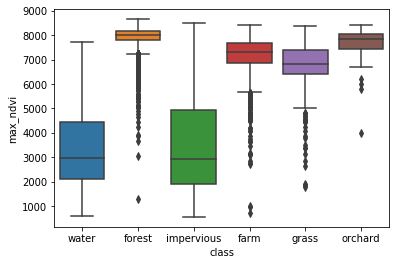
\includegraphics[width=0.20\textwidth]{figures/Analyse_exploratoire/boxplot_max-ndvi.png}}}%
    \qquad
    \subfloat[ NDVI minimum]{{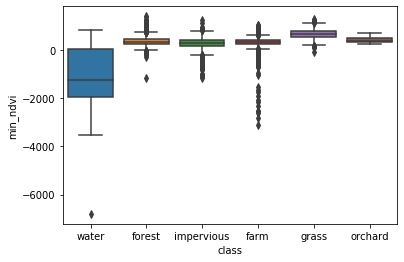
\includegraphics[width=0.20\textwidth]{figures/Analyse_exploratoire/boxplot_min-ndvi.png} }}%
    \vskip\baselineskip
    \subfloat[ Moyenne NDVI]{{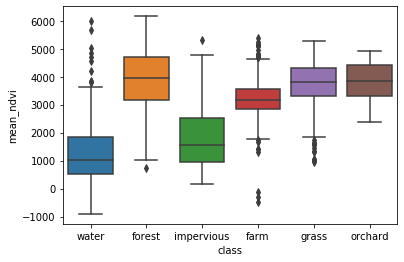
\includegraphics[width=0.20\textwidth]{figures/Analyse_exploratoire/boxplot_mean-ndvi.png}}}%
    \qquad
    \subfloat[ Écart-type NDVI]{{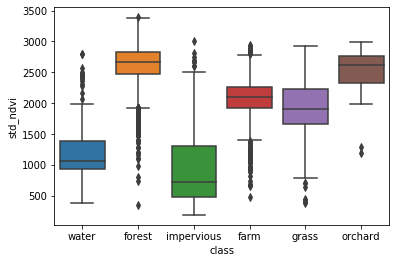
\includegraphics[width=0.20\textwidth]{figures/Analyse_exploratoire/boxplot_std-ndvi.png} }}
    \caption{\label{fig:ndvi}Figure non optimisée qui représente la répartition des valeurs NDVI en fonction des différentes classes}
\end{figure}


Ceci nous permet d'avoir un aperçu très global des différents types de valeurs que nous pouvons attendre pour chaque type de catégorie. Pour des terrains comme l'eau, le reflet de la lumière est assez faible, ce qui explique l'obtention de résultats NDVI maximum de niveau bas comparés à d'autres. De même pour les zones imperméables. 

Les mesures NDVI sont influencées par la présence de nuages ou non et peuvent causer l'enregistrement de données bruitées. Les saisons sont aussi des éléments qui influencent énormément les zones comme les fermes, les forêt, les pelouses ou encore les vergers. La végétation évolue en fonction des températures et des saisons. Pendant l'hiver et l'automne, le NDVI aura tendance à diminuer alors que pendant l'été et le printemps les valeurs seront beaucoup plus élevées. La figure~\ref{fig:season} mets en avant les 3 saisons en 2015 avec l'été en juin, le printemps en mai et l'hiver en janvier ainsi que les 4 saisons en 2014 avec l'automne en novembre, l'été en juin, le printemps en avril et l'hiver en janvier. 

\begin{figure}[htbp]
\begin{center}
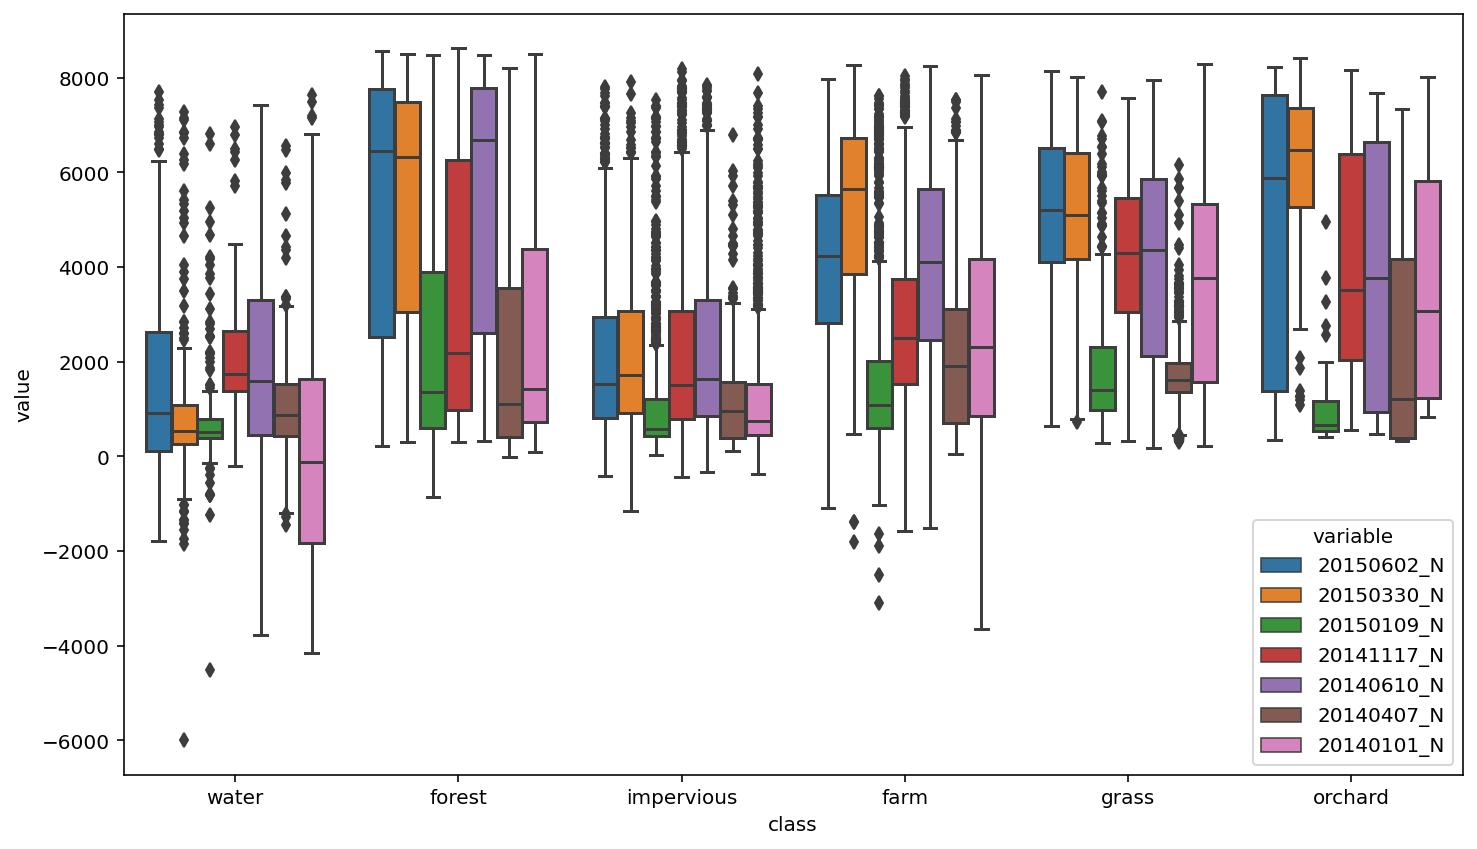
\includegraphics[width=0.45\textwidth]{figures/Analyse_exploratoire/box_plot_season.png}
\caption{\label{fig:season}Figure représentant le domaine pris des valeurs NDVI en fonction des classes et des saisons des années 2015 et 2014}
\end{center}
\end{figure}

Afin d'avoir un point de vue plus profond sur la tendance des valeurs NDVI en fonction du temps et des classes, nous avons regroupé les données de terrain par rapport à leurs classes. La figure \ref{fig:tendance_all} représente le changement de la moyenne de chaque classe (en ligne continue) en fonction du temps, et des quantiles $5\%$ et $95\%$ (en ligne pointillée).

Nous pouvons constater qu'il a y un pic en janvier de première année, ainsi qu'un autre pic en janvier de deuxième année. Nos données sont clairement périodiques, on pourra donc utiliser les outils d'analyse des séries temporelles périodiques pour dégager des caractéristiques intéressantes. 

\begin{figure}[htbp]
	\begin{center}
		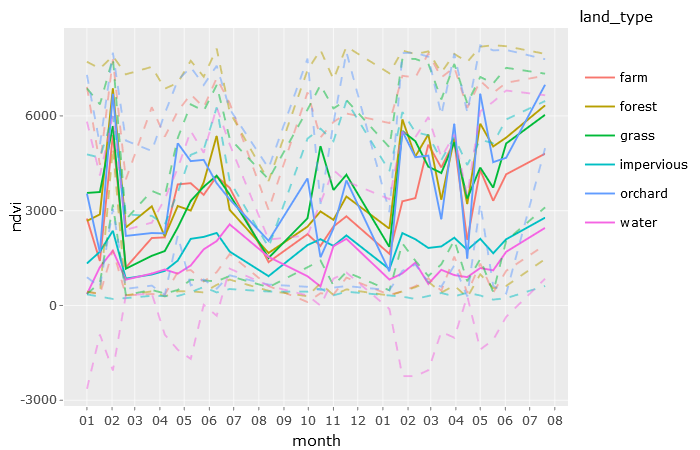
\includegraphics[width=0.45\textwidth]{figures/Analyse_exploratoire/tendance_all.png}
		\caption{\label{fig:tendance_all}Figure représentant la tendance de NDVI de chaque type de terrain}
	\end{center}
\end{figure}

Les tendances et les moyennes de classes forest, farm, grass et orchard semblent similaires ce que la figure \ref{fig:tendance_forest_grass_farm_orchard} montre, mais le nombre d'individus de chaque classe n'est pas équilibré. Cela peut potentiellement être un problème de classification déséquilibrée. 

\begin{figure}[htbp]
	\begin{center}
		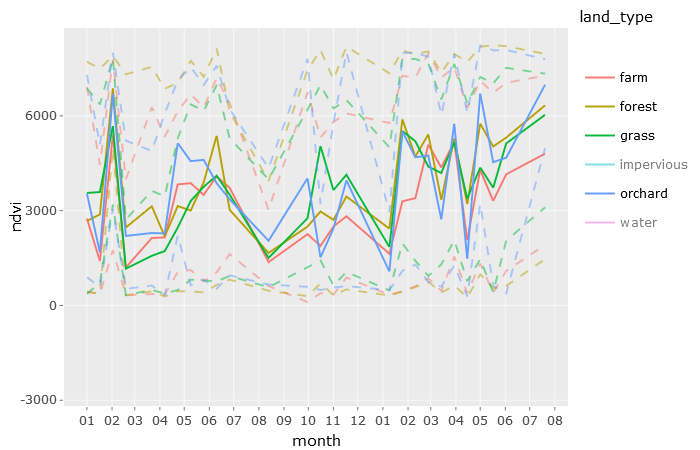
\includegraphics[width=0.45\textwidth]{figures/Analyse_exploratoire/tendance_forest_grass_farm_orchard.png}
		\caption{\label{fig:tendance_forest_grass_farm_orchard}Figure représentant la tendance de NDVI de chaque type de terrain}
	\end{center}
\end{figure}

Pour des catégories précises l'impact des saisons influence de manière très importante les valeurs mesurées de NDVI. En contre-partie pour certaines valeurs, on remarque une certaine stabilité malgré les changements de saison. 

Nous pouvons aussi utiliser l'analyse en composantes principales pour trouver les axes où les inerties expliquées qui sont les plus importantes. En obtenant les vecteurs propres on peut choisir les inerties expliqués suffisantes. Ici notre choix repose sur l'utilisation de la méthode du coude, mais nous aurions très bien pu utiliser un pourcentage d'inertie expliquée considéré comme suffisant. En cherchant à trouver la meilleure représentation des données, nous avons appliqué l'ACP plusieurs fois. La première fois sans aucune transformation. Pour la seconde en soustrayant à chaque colonne des individus l'axe dont l'inertie est la plus expliquée soit la valeur maximum du NDVI. Puis pour finir avec une réduction et un centrage sur les données avec suppression de l'axe maximum des NDVI. Pour chacun des cas, la méthode du coude a été appliquée, et dans la grande majorité, deux ou trois dimensions semblent convenir pour la représentation, comme l'indique la figure \ref{fig:ACP}
\begin{figure}[htbp]
\centering
    \subfloat[ ACP sans transformation ]{{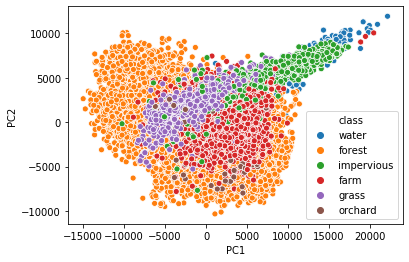
\includegraphics[width=0.20\textwidth]{figures/Analyse_exploratoire/ACP_normal.png}}}%
    \subfloat[ ratio d'inertie par Axe]{{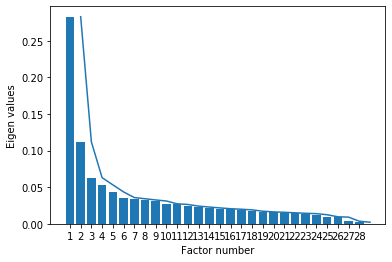
\includegraphics[width=0.20\textwidth]{figures/Analyse_exploratoire/ACP_normal_axe.png} }}%
    \vskip
    \subfloat[ACP en soustrayant l'axe le plus expliquée]{{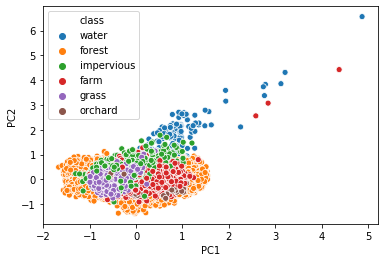
\includegraphics[width=0.20\textwidth]{figures/Analyse_exploratoire/ACP_noHighAxe.png} }}
    \subfloat[ ratio d'inertie par Axe]{{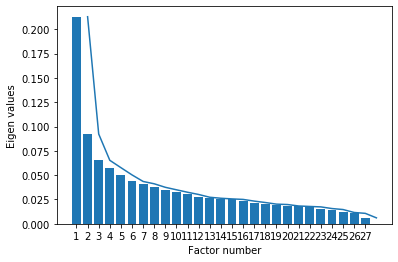
\includegraphics[width=0.20\textwidth]{figures/Analyse_exploratoire/ACP_noHighAxe_axe.png}}}%    
    \vskip
    \subfloat[ ACP avec valeurs centrées et réduites ]{{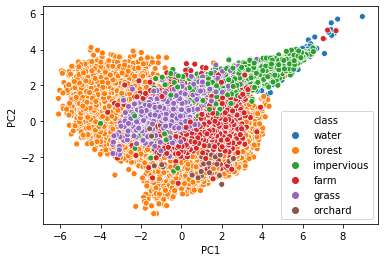
\includegraphics[width=0.20\textwidth]{figures/Analyse_exploratoire/ACP_centre_reduit.png}}}%
	\subfloat[ ratio d'inertie par Axe]{{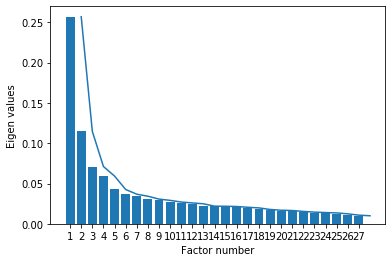
\includegraphics[width=0.20\textwidth]{figures/Analyse_exploratoire/ACP_centre_reduit_axe.png}}}%
    \caption{\label{fig:ACP}ACP avec utilisation de la méthode du coude}
\end{figure}

On remarque très rapidement que l'utilisation de l'ACP semble difficilement applicable sur ce jeu de données en grande dimension avec des phénomènes non-linéaires. Il est aussi intéressant de noter que l'ACP a une tendance à beaucoup moins bien se comporter pour la présence de valeurs extrêmes. Les résultats obtenus ne permettent pas de distinguer de manière flagrante les clusters des classes. Il est possible d'envisager d'améliorer cette représentation en utilisant une Analyse en Composant Principale par Noyau. Une autre approche pourrait être de réaliser cette ACP en supprimant les données d'images satellites dont les valeurs sont considérés aberrantes et les ajouter par la suite. De cette manière lors de la pondération de la formation des axes, ils influenceraient moins les choix des axes, et donc ils  n'auraient pas participer à la formation des axes.


%----------------------------------------------------------------------------------------
\section{Analyse Spectrale} 

Nous étudions des séries temporelles qui suivent des tendances périodiques dues aux saisons de l'année. Pour examiner les domaines de fréquences des séries temporelles, nous avons réalisé une analyse spectrale des données.
Grâce à la transformée de Fourier rapide, on obtient les coefficients de Fourier associés aux séries. Ces coefficients décrivent totalement les informations contenues dans les séries temporelles. Lorsque l'on applique un filtre passe-bas, on néglige les hautes fréquences et on obtient l'allure générale de la série. On obtient ainsi les tendances générales de la série comme on peut le voir sur la figure \ref{fig:fourier}.
\begin{figure}[htbp]
\begin{center}
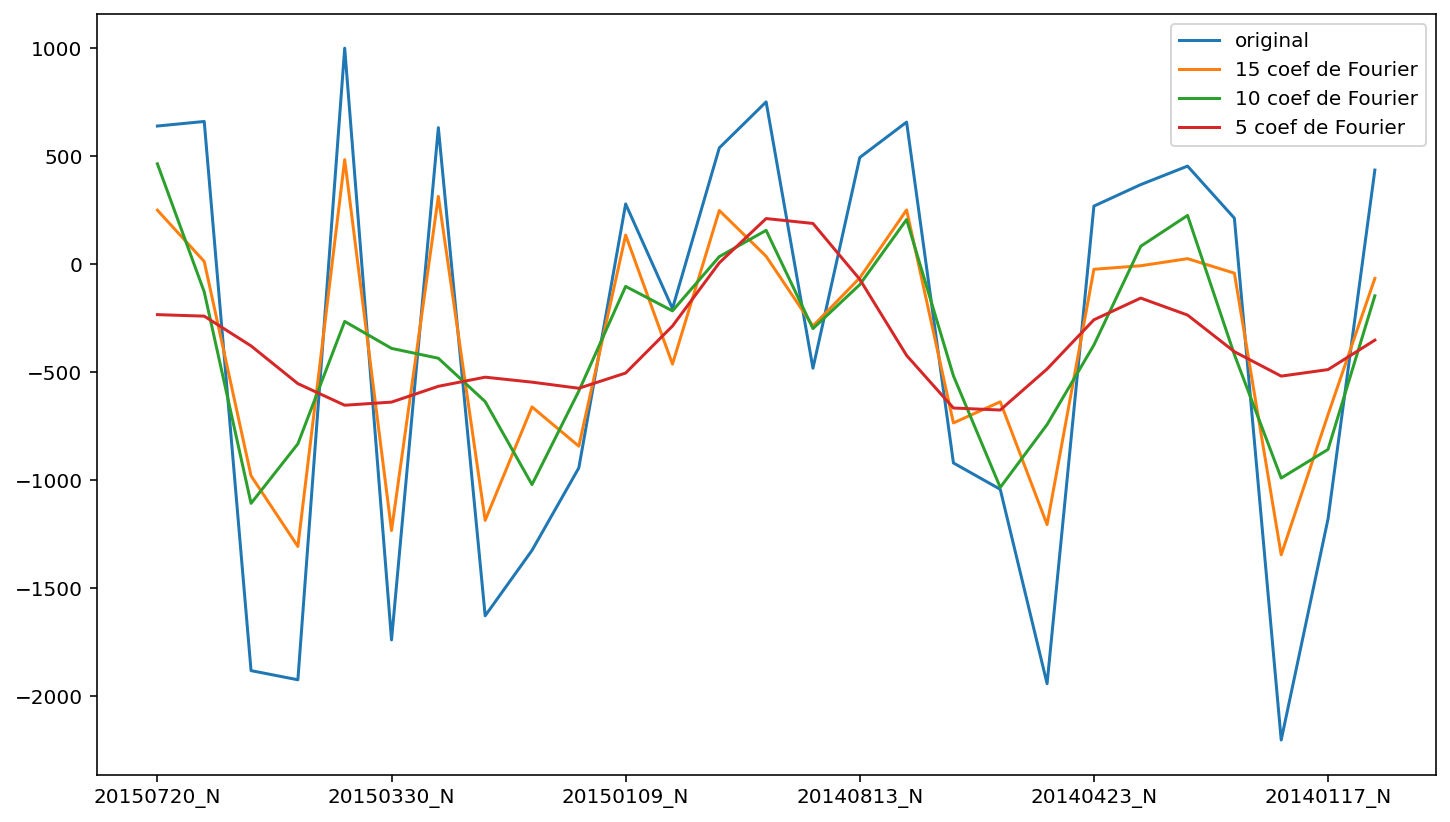
\includegraphics[width=0.45\textwidth]{figures/ift.png}
\caption{\label{fig:fourier}Les différentes reconstitution d'une série temporelle avec un filtre passe-bas de plus en plus accentué.}
\end{center}
\end{figure}

Pour obtenir les coefficients de la transformée de Fourier, on applique simplement l'algorithme de transformation de Fourier rapide.

Les coefficients sont calculés selon la formule suivante~:
\[
f_j =  \sum_{k=0}^{n-1} x_k e^{-\frac{2\pi i}{n} jk }
\]

Cette analyse spectrale est théoriquement un bon traitement préalable à la réduction de dimensionnalité : les hautes fréquences dans les mesures sont très probablement du bruit qu'il convient d'ignorer pour nos analyses. Lorsque l'on effectue une analyse en composante principale sur nos coefficients de Fourier (cf. Figure \ref{fig:acp_fourier}), on observe trois classes qui se dégagent, une classe imperméable, une classe pour l'eau et une autre classe où toutes les autres classes se mélangent. La forêt recouvre particulièrement une grande zone ce qui empêche de distinguer clairement les classes dans cette zone.

\begin{figure}[htbp]
\begin{center}
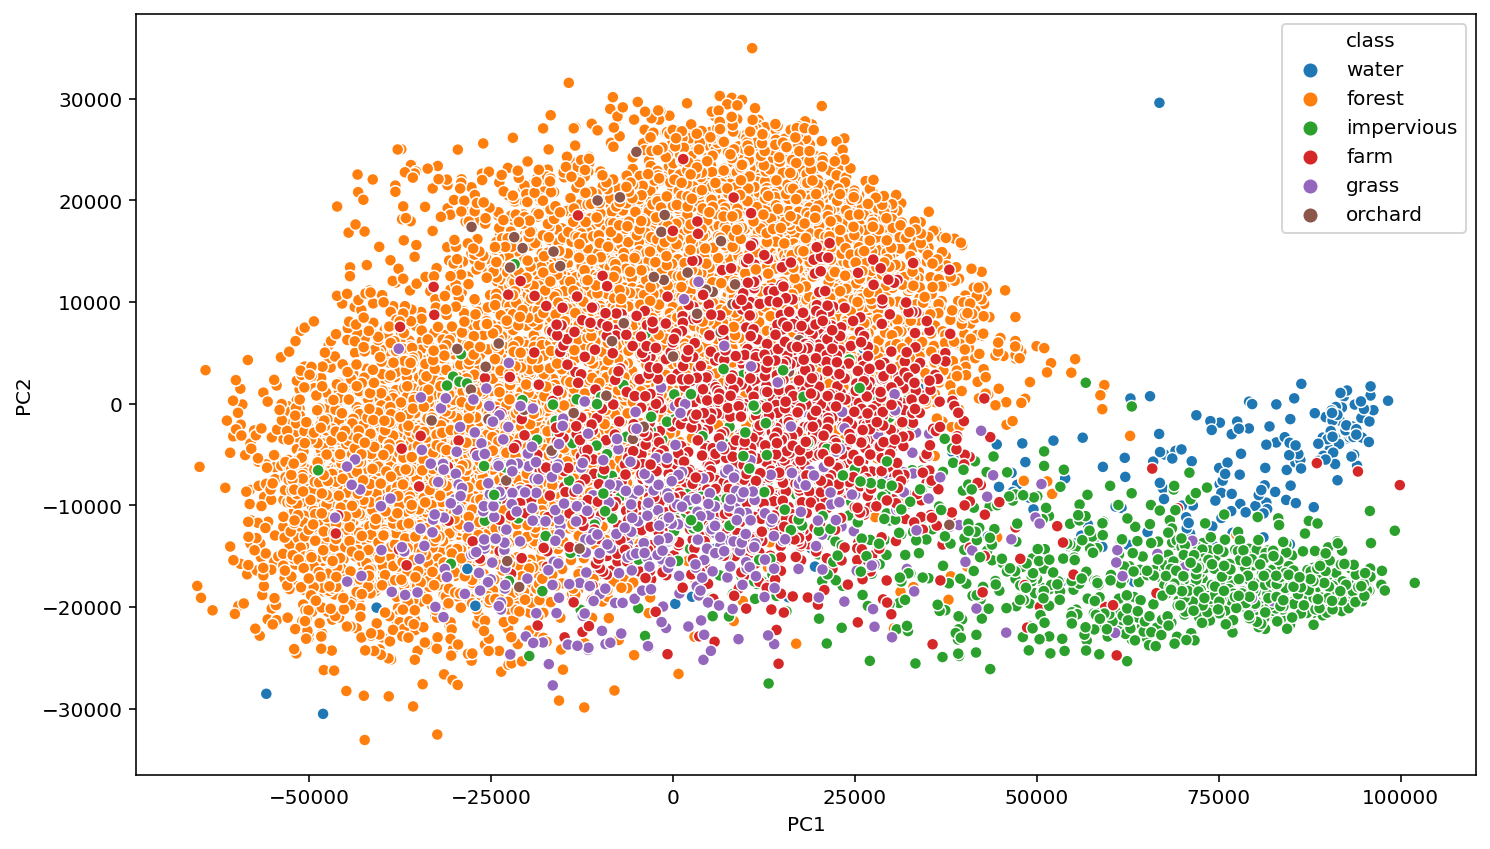
\includegraphics[width=0.45\textwidth]{figures/acp_fourier.png}
\caption{\label{fig:acp_fourier} Représentation des données sur les deux axes principaux dégagés par l'ACP}
\end{center}
\end{figure}

D'après les taux de variance expliqué (cf. Figure \ref{fig:explained_variance_fourier}), le premier axe explique beaucoup de variance mais à partir de la deuxième dimension, la variance expliquée est très répartie entre les dimensions ce qui n'aide pas à faire de réduction de dimensionnalité. L'analyse spectrale n'a donc pas permis de dégager des features particulièrement efficaces pour expliquer la variance des données. Nous verrons plus tard que travailler avec les coefficients de Fourier n'améliore pas la qualité des modèles de classification non plus.

\begin{figure}[htbp]
\begin{center}
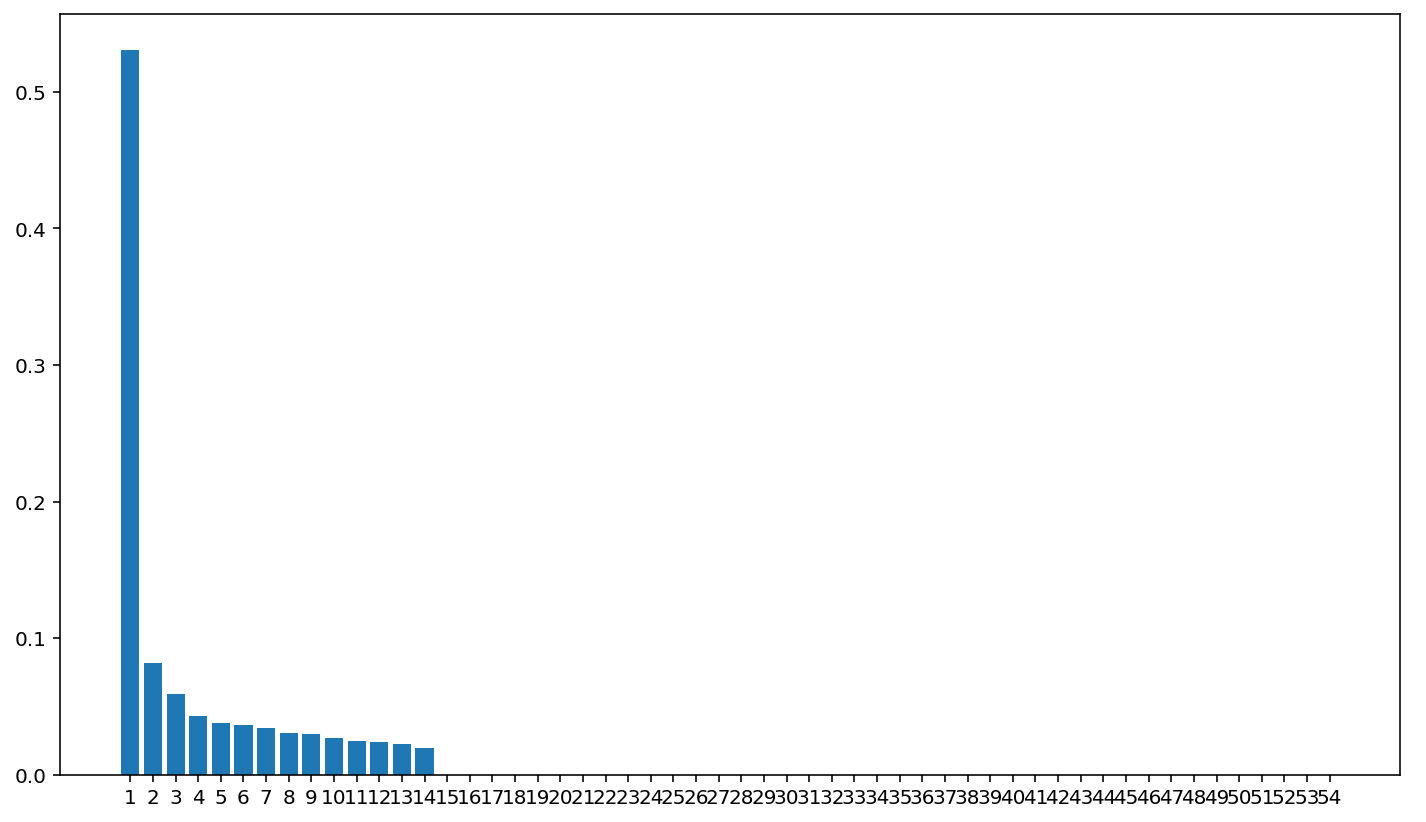
\includegraphics[width=0.45\textwidth]{figures/explained_variance_fourier.png}
\caption{\label{fig:explained_variance_fourier}Les taux de variance expliqué selon le nombre de dimensions conservées.}
\end{center}
\end{figure}





%----------------------------------------------------------------------------------------
\section{Apprentissage} 

L'étude d'images satellites va s'effectuer sur trois types de jeu de données. Un jeu de données (Training dataset) sera utilisé pour l'apprentissage de la classification des données, ensuite le second jeu de données (Validation dataset) permet de trouver les meilleurs hyperparamètres et aussi d'évaluer si notre modèle sélectionné est bien approprié pour nos données. Le troisième jeu de données (Test dataset) est consacré seulement à évaluer la performance de notre classifieur qui est bien configuré en utilisant les données d'apprentissage. Parmi les différentes méthodes d'apprentissage des données, nous allons retenir celles avec les meilleurs résultats tout en limitant \textit{l'over-fitting} (sur-apprentissage). Nous allons considérer que notre jeu de données d'apprentissage est suffisamment grand avec 10545 images pour pouvoir réaliser des séparations et construire des jeux de données pour la validation qui sont de petites tailles. 

\begin{figure}[htbp]
\begin{center}
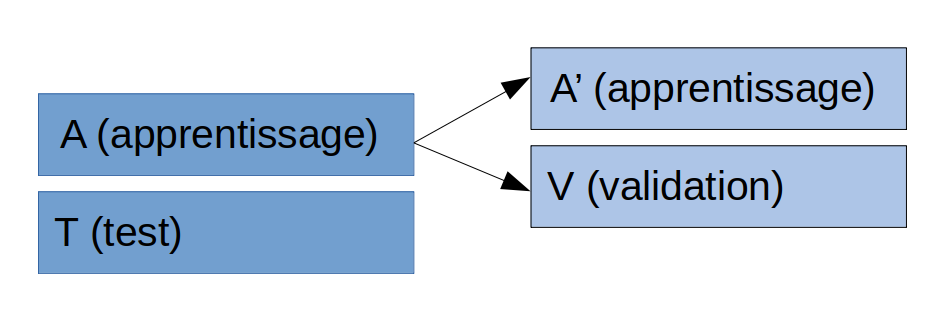
\includegraphics[width=0.45\textwidth]{figures/jeu_de_donnees.png}
\caption{\label{fig:jeu_de_données}Jeux de données utilisées pour l'apprentissage}
\end{center}
\end{figure}

Parmi les différentes méthodes d'apprentissage vues en cours, deux grandes catégories existent, l'apprentissage non-supervisé et l'apprentissage supervisé. Pour le premier cette classification repose sur la structure inhérente des données en entrées, alors que pour le second c'est sur la reconnaissance des formes et sur l'étiquetage des données pour ensuite établir un système de prédiction. 

La méthode appliquée ici pour classifier et apprendre sur les images satellites va reposer sur la méthodologie de construction d'une règle de décision. Nous avons notre ensemble de données pour l'apprentissage et de tests. Nous avons aussi réalisé le choix des variables pour décrire une image. Il suffit d'appliquer les différentes méthodes et de garder les modèles qui ont eu une évaluation des performances les plus élevées. Cependant il faut sélectionner une ou des règles de décision qui permettent de vérifier cette apprentissage et d'obtenir des performances satisfaisantes. Il faut éviter les risques de sur-apprentissage lors des choix des hyper-paramètres, l'un des grands risques avec la présence de données bruités dans notre jeu et bien généraliser cette apprentissage. 

\subsection{Classification ascendante hiérarchique}
La méthode classification ascendante hiérarchique va calculer la distance entre chaque paire d'individus, et regrouper les deux individus dont la distance est la plus proche dans une classe (cluster). Ensuite, elle groupe de la même façon les deux classes dans une classe plus grande. C'est une procédure par regroupement successive en partant des singletons. Une méthode plus généralement utilisé que la classification descendante, qui procède par division successive. Dans le cas des images satellites, il est plus facile de regrouper en se basant sur les ressemblance.  

La méthode de mesure pour la distance entre des classes différentes peut être définie par plusieurs possibilités. L'avantage de cette méthode est qu'elle est facile à appliquer avec des méthodes de mesure prédéfinies. Il suffit de trouver une bonne méthode de mesure pour la distance comme c'est un modèle non supervisé. Par contre, sa complexité de calcul est relativement élevée, et il est moins performant pour des données ayant une inertie interclasse trop petite et une inertie intraclasse trop grande surtout dans notre cas.

Nous avons donc évalué ce modèle par l'indice de rand ajusté, et nous avons obtenu, en utilisant la méthode de Ward, le meilleur score de $13\%$ pour le jeu de données de l'apprentissage. Malheureusement, ce n'est pas suffisant pour être un bon modèle d'apprentissage pour nos données.

\begin{figure}[htbp]
	\centering
		\subfloat[Classification avec méthode ward ]{{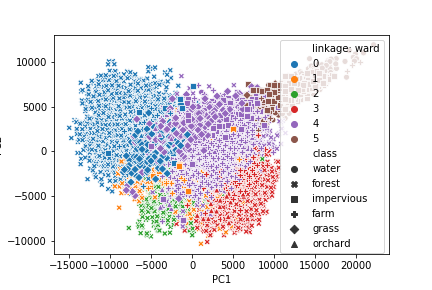
\includegraphics[width=0.20\textwidth]{figures/CAH/ward.png}}}%
		\subfloat[Hiérarchie avec niveau de profondeur == 4]{{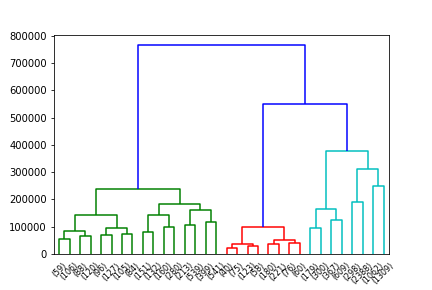
\includegraphics[width=0.20\textwidth]{figures/CAH/hierarchie.png} }}%
\end{figure}
 
Cette classification non supervisé est difficile. Trouver une bonne classification des images satellites c'est trouver une classification de groupes homogènes, à l'aide de mesure de similarité mais pour certaines étiquettes de notre jeux de données, les terrains ont des comportement très similaire et son difficilement dissociable. 

\subsection{K-Means}
La méthode des centres mobiles peut être réalisée sur $p$ variables quantitatives. Il suffira pour cela d'ignorer l'étiquetage des données sur le type de terrain. On associe à chaque image satellite une représentation dans l'espace $\mathcal{R}^n$ muni d'une pondération $\frac{1}{n}$. Dans notre cas on connait au maximum le nombre de cluster à trouver ici qui représente les différentes catégories définis pour un terrain : \pycode{k = len(set(x["class"]))} avec $k=6$. 
L'objectif est d'affecter le point au centre de la classe le plus proche. Cette algorithme va être itéré jusqu'à obtenir des centres de classes stables d'une itération à l'autre avec le même effectif. 

Pour évaluer l'efficacité de ce modèle, il va falloir comparer les deux partitions entre-elles, la partition obtenu avec la méthode des "K-means" et la partition des classes obtenue avec l'étiquetage. Ici la proximité des deux partitions ne peut être calculée directement avec une correspondance entre les deux qui n'est pas bien identifiée. Pour y faire face, il est possible d'utiliser l'indice de rand, qui va mesure la similarité entre deux partitions avec le dénombrement des paires d'éléments. On va utiliser l'indice de rand ajusté qui permet d'éviter de tendre vers 1 asymptotiquement quand le nombre de partitions augmente, même si ici, le nombre est peu élevé et fixe. Le résultat obtenu est de $10\%$ avec le jeu de données pour l'apprentissage et de $30\%$ pour le jeu de test. Ici l'apprentissage est non supervisé donc le faire sur l'un ou l'autre n'a pas de conséquence, en contre-partie, on remarque sur des gros jeux de données, l'algorithme se comporte beaucoup moins bien. 

\begin{figure}[htbp]
\begin{center}
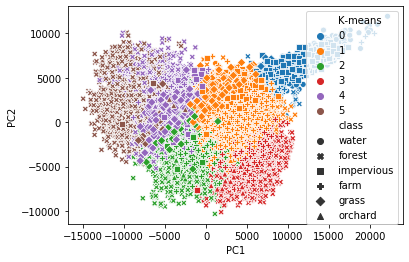
\includegraphics[width=0.45\textwidth]{figures/k-means.png}
\caption{\label{fig:k-means}Résultat obtenu avec la méthode des k-means comparé aux étiquettes}
\end{center}
\end{figure}


\subsection{K plus proche voisin}
Dans un premier temps il est possible de comparer très rapidement les frontières obtenues avec différentes méthodes avec une représentation des données en composantes principales. L'ACP utilisée est celle de base sans transformation. Il est nécessaire de diminuer les dimensions de représentation pour pouvoir afficher visuellement les frontières en deux dimensions.  

\begin{figure}[htbp]
\begin{center}
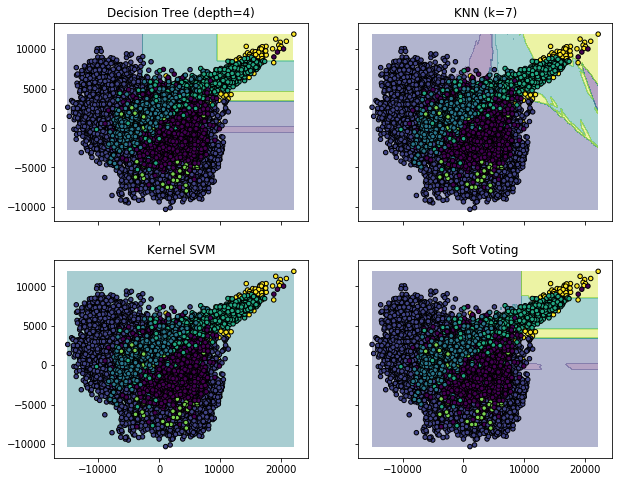
\includegraphics[width=0.45\textwidth]{figures/ACP_learningAlgo.png}
\caption{\label{fig:ACP_learningAlgo}Les frontières calculé par l'utilisation de différentes méthodes}
\end{center}
\end{figure}

On remarque très rapidement que la méthode de l'arbre de décision et des $k$ plus proches voisins semblent être mieux adaptés pour ce type de jeu de données. Il faut toutefois nuancer ce résultat obtenu à partir d'une transformation des données pour s'adapter à cette représentation. 

L'algorithme des $K$ plus proches voisins n'a pas vraiment de phase d'apprentissage, on ne règle pas vraiment de paramètre.Ce qui influence la qualité d'évaluation du modèle est le choix du nombre de voisin $k$. Pour obtenir le meilleur $k$ il existe différentes méthodes. Si le $k$ choisi est trop petit alors l'algorithme risque de trop s'adapter aux données et si le $k$ est trop grand, l'algorithme risque de trop généraliser. Il va falloir trouver un compromis entre les deux qui nous permet d'obtenir les meilleurs taux de validation. La première méthode utilisé pour trouver le $K_{opt}$ est de séparer le jeu de données d'apprentissage en deux groupes, avec $\frac{9}{10}$ des données comme données d'apprentissage et le reste comme données de validation. En réalisant le test sur différents $k$, on va chercher celui qui permet d'obtenir le meilleur résultat. La courbe qui illustre le résultat obtenu dans la figure \ref{fig:k_plus_proche_voisin} est celle pour $K_{opt}=1$. La seconde solution pour trouver le meilleure $K_{opt}$ s'adapte mieux lorsque l'espace hypermétrique est très grand. La validation simple obtenue peut avoir sélectionné le mauvais modèle. Nous allons donc utiliser une validation multiple en réalisant plusieurs apprentissages simples en changeant à chaque itération l'ensemble de validation et l'ensemble d'apprentissage. On utilise pour la recherche la fonction \pycode{GridSearchCV} qui permet d'appliquer la validation croisée. La courbe qui illustre cette nouvelle méthode est sur la figure \ref{fig:k_plus_proche_voisin} avec $K_{opt}=9$. Pour chacun des tests on sélectionne le $K$ qui permet d'obtenir le meilleur score de validation	. Il est intéressant de noter que les deux $K_{opt}$ obtenus sont des nombres impairs pour éviter les ex aequo. 

\begin{figure}[htbp]
\centering
    \subfloat[ $K_{opt} = 1$ ]{{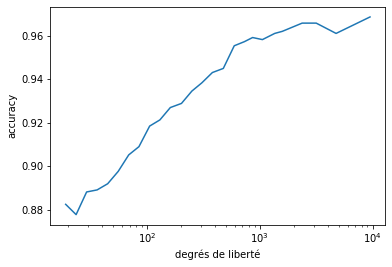
\includegraphics[width=0.20\textwidth]{figures/k_plus_proche_k=1.png}}}%
    \qquad
    \subfloat[ $K_{opt} = 9 $ ]{{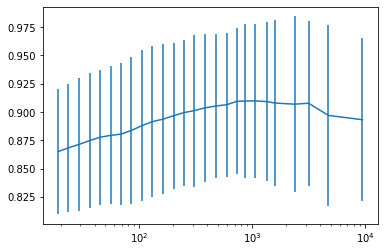
\includegraphics[width=0.20\textwidth]{figures/k_plus_proche_k=9.png} }}%
    \caption{Évolution de la validation en fonction du degré de liberté sélectionnée $k$}%
    \label{fig:k_plus_proche_voisin}%
\end{figure}

En testant chacun des $K_{opt}$ obtenu, on obtient un score de performance du modèle de $62.3\%$ pour $K_{opt} = 9$ et $58.6\%$ pour $K_{opt} = 1$. Cela confirme bien que la seconde méthode est préférable lorsque l'espace paramétrique est très grand. 

%TODO : Gradiant et ACP ... 

\subsection{Analyse discriminante}
En utilisant un apprentissage supervisé, nous allons appliquer la méthode naïve de Bayes, l'analyse discriminante quadratique et l'analuse discriminante liénaire. Par contre le jeu de données utilisé dans ce cas à été modifié par une méthode de gradiant pour prendre en compte la dispersion des données NDVI dans le temps. Pour l'appliquer nous avons soustrait la colonne par sa colonne de gauche. Ensuite avec ce jeu de données modifié nous avons appliqué les différentes méthodes, résumées dans le tableau ci-contre : 

\begin{table}[h]
\caption{Résultat des performances des différntes méthodes}
\begin{tabular}[t]{l|l}
 \textbf{Linear Discriminant Analysis} &   59.33\%\\
 \textbf{Quadratic Discriminant Analysis} &    44.33\% \\
 \textbf{Guassian NB} &  70.00\%\\
\end{tabular}
\end{table}

Pour le test linéaire, des tests de validation ont été réalisés pour sélectionner les meilleurs paramètres parmi trois solveurs : \pycode{svd}, \pycode{lsqr}, ou \pycode{eigen}. Parmi les trois, c'est le \pycode{svd} qui obtient les meilleurs résultats. Cette méthode repose sur une analyse des décompositions singulières des valeurs et se comporte très bien pour les jeux de données en gros volume de paramètres, ce qui est notre cas. Les deux autres méthodes peuvent être combinées avec une méthode de shrinkage pour réduire les effets d'échantillonnage des variables. 

La méthode discriminante linéaire peut aussi être utilisée pour réduire la dimension des données en utilisant les directions discriminantes. Dans le cas de l'ACP c'est un apprentissage non supervisé qui ignore les catégories labellisées et qui maximise la variance des données. En contre-partie dans le cadre du LDA on prend en compte les classes et on cherche les axes qui maximisent la séparation entre les catégories. Pour réaliser cette transformation on applique \pycode{fit} ,\pycode{transform} qui peut aussi être combiné avec l'outil \pycode{StandardScaler} qui permet de centrer et réduire les données en utilisant la moyenne et l'écart-type comme le montre la figure \ref{fig:LDA}. Néanmoins même en appliquant d'autres méthodes sur cette nouvelle représentation, les résultats n'ont pas été concluants. Par exemple pour les K plus proches voisins on obtient un niveau de performance de 53\%. sur les données de tests qui ont subit les mêmes transformations aussi. 

\begin{figure}[htbp]
\centering
    %\subfloat[ Réprésentation en 2 dimensions ]{{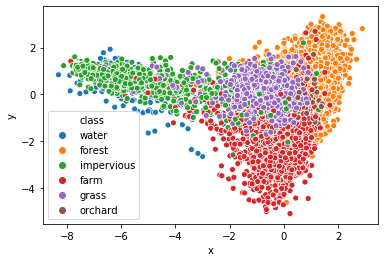
\includegraphics[width=0.20\textwidth]{figures/LDA-QDA-Naive/LDA_dim.png}}}%
    %\qquad
    \subfloat[ Frontière de décision avec K plus proches voisins $K_{opt}=31$  ]{{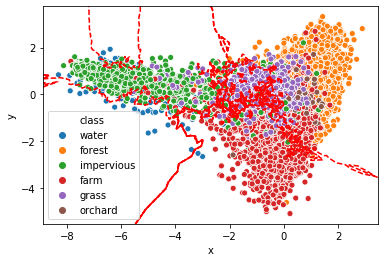
\includegraphics[width=0.20\textwidth]{figures/LDA-QDA-Naive/LDA_dim_bound.png} }}%
    \qquad
    \subfloat[ Frontière de décision avec K plus proches voisins sur le jeu de test ]{{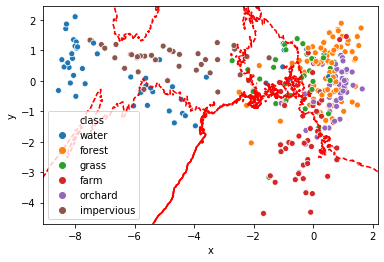
\includegraphics[width=0.20\textwidth]{figures/LDA-QDA-Naive/LDA_test.png} }}
    \caption{Réduction de la dimension du jeu de données avec l'analyse discriminante linéaire et une réduction et centrage des données}%
    \label{fig:LDA}%
\end{figure}

Nous avons ensuite appliqué la méthode naïve de Bayes. La règle de Baye est une règle de décision qui consiste à minimiser les probabilités d'erreurs. On affecte le point à la classe qui à la plus grande probabilité à posteriori. Par contre pour la réalisation de ce test, nous n'appliquons pas la notion de risque. Ici les données ne présentent pas de réelle risque si on en choisit une plutôt que l'autre. En contre partie, si notre jeu était sur des données médicales avec des individus malade ou non, la question de risque est beaucoup plus cruciale. La méthode naïve de Bayes est un apprentissage qui ne nécessite pas la recherche d'hyperparamètres et peut être appliquée directement. L'avantage d'appliquer l'algorithme de la méthode naïve de Bayes est qu'il se comporte très bien sur de gros jeu de données et c'est un algorithme robuste et fiable. Néanmoins, pour pouvoir l'appliquer, on doit supposer que les variables sont indépendantes entre-elles mêmes si ici ce n'est pas vraiment le cas. Dans la figure \ref{fig:NaiveBayes} on peut analyser la répartition des données dans les classes ou la meilleure probabilité a été trouvé grâce à la formule de Bayes avec les probabilité à priori calculé avec l'étiquetage lors de l'apprentissage. 

\begin{figure}[htbp]
\begin{center}
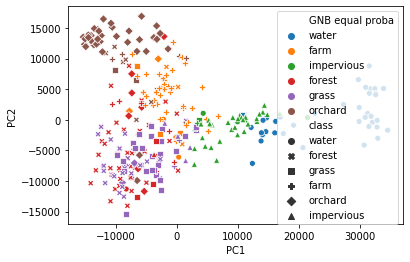
\includegraphics[width=0.45\textwidth]{figures/LDA-QDA-Naive/NaiveBayes.png}
\caption{\label{fig:NaiveBayes}Évaluation des performances de l'algorithme Naïf de Bayes}
\end{center}
\end{figure}


\subsection{Arbres de décision et méthodes ensemblistes}
En créant un simple arbre de décision sur nos données de façon naïve, on obtient un modèle qui a sur-appris : le modèle classifie correctement tous les échantillons de notre jeu d'apprentissage, mais il généralise mal et a une précision de 0.56 sur le jeu de test. 

De plus, le résultat de gain d'information est facilement influencé par le nombre d'individus de chaque classe. Autrement dit, la classe qui possède le plus grand nombre d'individus aura un plus grand taux de classification que les autres classe. Particulièrement dans notre cas, nous avons $ 7431 $ individus de classe forêt et $ 53 $ individus de classe verger.

La méthode des forêts aléatoires généralisent un peu mieux et culminent à une précision de 0.63 pour une dizaine d'arbres.

La matrice de confusion \ref{confusion_matrix} illustre bien les observations que l'on avait pu faire lors de l'ACP : la classe forêt recouvre une large zone et empêche de classifier correctement les fermes, les prairies et les vergers (cf. Figure \ref{fig:acp_fourier}).

\begin{table}[h]
	\caption{Matrice de confusion d'une forêt aléatoire sur les données brutes}
	\label{confusion_matrix}
	\begin{tabular}{l|llllll}
		        & E  & F  & I  & A  & P & V \\ \hline
		Eau     & 34 & 2  & 3  & 6  & 1 & 0 \\
		Forêt   & 0  & 69 & 1  & 6  & 2 & 0 \\
		Imper   & 0  & 1  & 36 & 2  & 1 & 0 \\
		Agri    & 0  & 11 & 0  & 42 & 0 & 0 \\
		Prairie & 0  & 19 & 3  & 6  & 8 & 0 \\
		Verger  & 0  & 43 & 0  & 4  & 0 & 0
	 \end{tabular}
\end{table}

Les coefficients de Fourier que l'on avait trouvés pour l'analyse spectrale ne permettent pas d'obtenir de meilleurs modèles. Au contraire, les forêts ne parviennent plus qu'à atteindre une précision de 0.5 lorsqu'elles apprenent du jeu de donnée spectral.

Nous avons aussi essayé d'appliquer ce modèle sur le jeu de données original et le jeu de données transformé par l'ACP pour avoir une précision plus élevé. Malheureusement, notre classifieur n'atteint qu'une précision $54\%$.

\begin{figure}[htbp]
	\centering
	\subfloat[ training set ]{{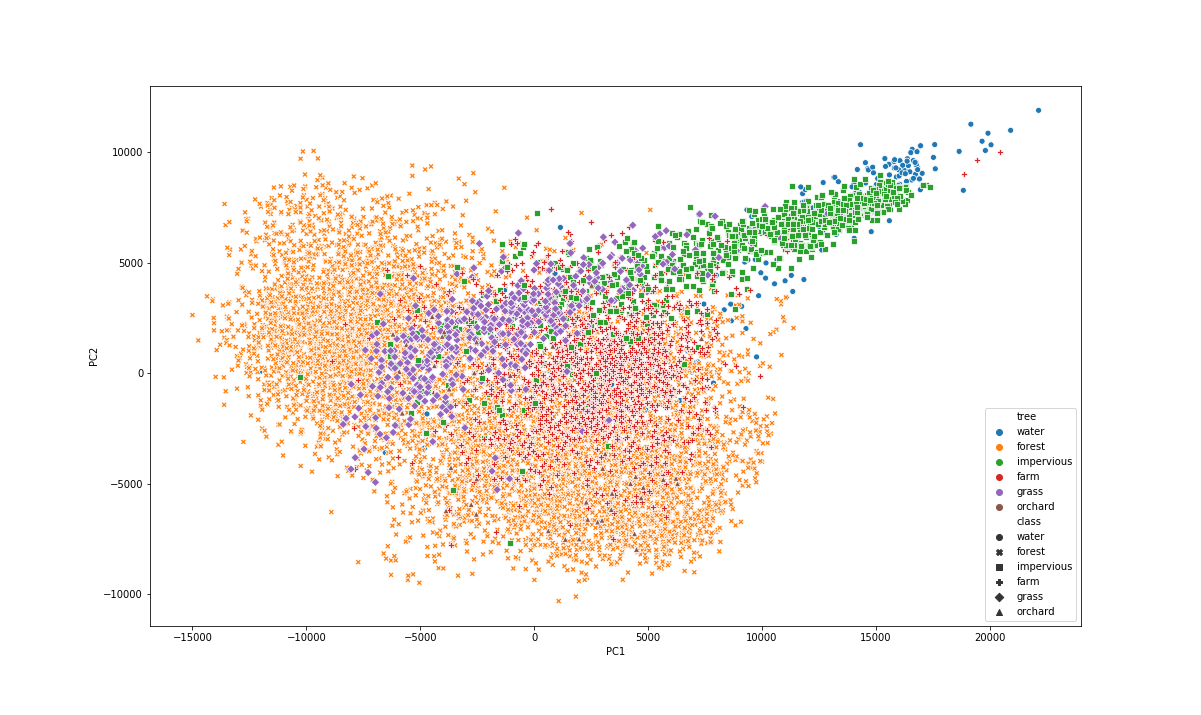
\includegraphics[width=0.20\textwidth]{figures/Tree/decisiontree_training.png}}}%
	\qquad
	\subfloat[ testing set ]{{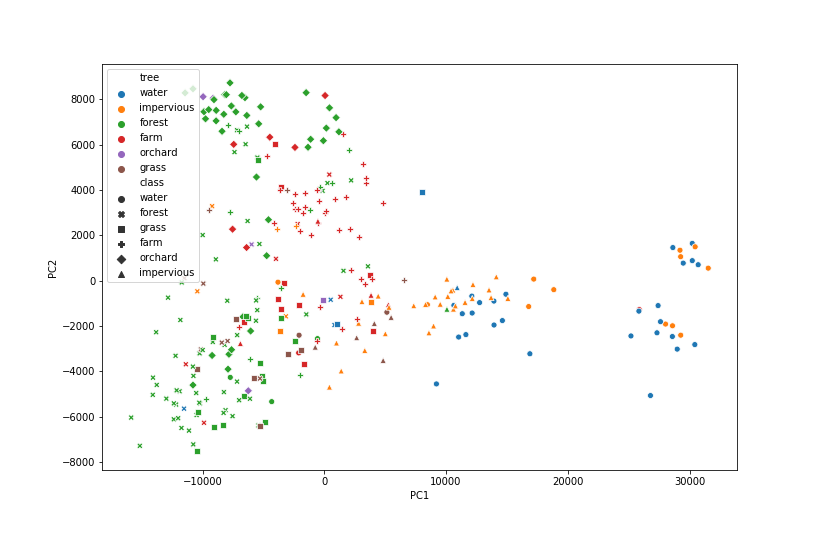
\includegraphics[width=0.20\textwidth]{figures/Tree/decisiontree_testing.png} }}%
	\caption{Prédiction par l'arbre de décision}%
	\label{fig:DTree}%
\end{figure}

En analysant les résultats que nous avons obtenus, nous avons trouvé que ce modèle ne génère qu'un seul arbre. Par conséquent, le processus de calcul est simple et c'est donc plus compréhensible pour nous et moins coûteux pour l'ordinateur. Au contraire, il est beaucoup facile d'avoir un sur-apprentissage, ainsi qu'il est moins puissant de récupérer les informations du rapport entre des variables. En plus, le résultat de gain d'information est facilement influencé par le nombre d'individus de chaque classe. Autrement dit, la classe qui possède le plus grand nombre d'individus aura un gain plus grand par rapport aux autres classe, cela amènera a de plus grand possibilité de classifier mal sur la classe qui possède moins d'individus. Particulièrement dans notre cas, nous avons $ 7431 $ individus de classe forêt et $ 53 $ individus de classe verger. Comme nous avons constaté précédemment, il existe des similarités de tendance et de moyenne entre ces deux classes, le résultat de prédiction \ref{confusion_matrix} ( la plupart de verger est considéré comme forêt) est donc raisonnable et logique.

Ce jeu de données semble favoriser plus encore la classification massive en forêt aléatoire (random forest). Le modèle de forêt aléatoire est performant et évite le sur-apprentissage bien qu'il soit plus coûteux qu'un arbre simple. D'ailleurs, afin de rendre compte des poids de classe, nous retirons aléatoirement des individus de nombre identique depuis chaque classe. La taille du jeu de l'apprentissage est par conséquent limité par la taille de la classe qui contient le moins d'individus. En conséquence, il y aura un sous-apprentissage (underfitting), c'est à dire que tout le jeu d'apprentissage n'est pas utilisé. Pour résoudre ce problème, nous faisons $ 1000 $ répétitions du modèle forêt aléatoire avec classes équilibrées, pour ensuite effectuer une classification par jugement majoritaire. Cela s'apparente à un vote de 1000 personnes, le résultat sera la classe qui aura le plus grand nombre de bulletins de vote. Même si chaque forêt prend peu de données, la plupart de données seront utilisées au moins une fois après un grand nombre de répétitions. Cette méthode fonctionne bien avec un score de performance de $ 72\% $.

\begin{figure}[htbp]
	\begin{center}
		\label{fig:randomforest}
		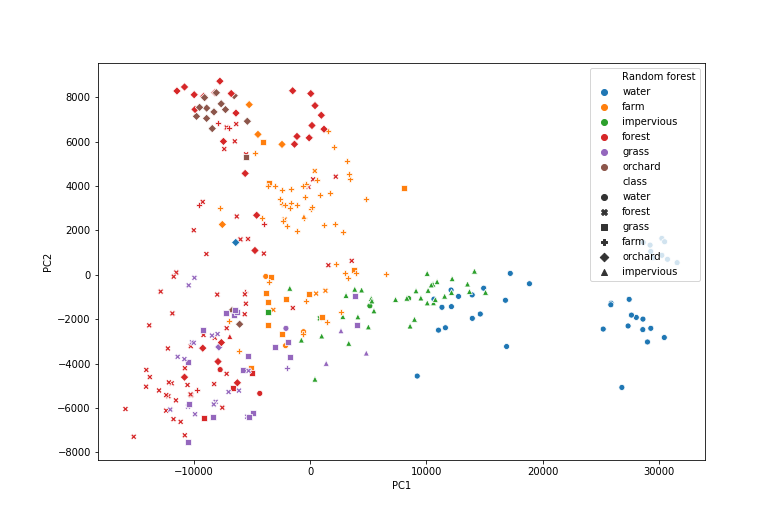
\includegraphics[width=0.45\textwidth]{figures/Tree/randomforest_repetition.png}
		\caption{1000x Random Forest}
	\end{center}
\end{figure}

Au contraire de la classification d'une seul forêt aléatoire (Table \ref{confusion_matrix}) où une grande part des individus de la classe farm, orchard et grass sont considérées comme la classe forêt dans sa prédiction, il y a une amélioration de précision (Table \ref{confusion_matrix_1000xforeset}) pour ces classe de minorité dans la classification de 1000 forêts aléatoires.

\begin{table}[h]
	\caption{Matrice de confusion de 1000 répétition de forêt aléatoire sur les données brutes}
	\label{confusion_matrix_1000xforeset}
	\begin{tabular}{l|llllll}
		           & Fa. & Fo. & Gr. & Im. & Or. & Wa. \\ \hline
		Farm       & 46   & 5      & 2     & 0          & 0       & 0     \\
		Forest     & 5    & 51     & 21    & 0          & 1       & 0     \\
		Grass      & 11   & 3      & 19    & 1          & 2       & 0     \\
		Impervious & 1    & 1      & 0     & 38         & 0       & 0     \\
		Orchard    & 2    & 23     & 1     & 0          & 20      & 1     \\
		Water      & 3    & 1      & 2     & 2          & 0       & 38
	\end{tabular}
\end{table}


Nous avons aussi appliquer comme autre méthode l'élagage d'un arbre, en espérant obtenir de meilleurs résultats pour le taux d'évaluation du modèle. Cette méthode consiste à construire l'arbre complet puis couper les branches (élaguer) pour simplifier le modèle et s'assurer que le modèle généralise bien les données et empêcher l'over-fitting. Pour trouver les branches à élaguer, il faut cherche le meilleure $\lambda$ qui permet de régler le compromis en considérant le cout et la complexité du jeu de données à apprendre. Pour valider le meilleurs hyper-paramètres nous utilisons la méthode de validation croisée pour changer à chaque itération le bloc d'apprentissage et le bloc de validation et ainsi varier cette subdivision. La figure \ref{fig:elagage} permet d'illustrer les erreurs de validations obtenus avec différents $\lambda$. Dans notre cas on obtient $\lambda_{opt} = 0.00024$ qui permet ensuite d'appliquer l'élagage à notre arbre de décision. Et finalement le taux d'évaluation obtenus du modèle est de $56\%$.

 
\begin{figure}[htbp]
	\begin{center}
		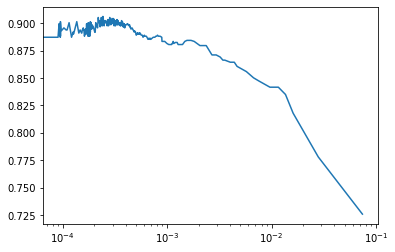
\includegraphics[width=0.45\textwidth]{figures/Tree/elagage.png}
		\caption{\label{fig:elagage}Erreurs de validation en fonction des $\bar{\lambda_k}$} 
	\end{center}
\end{figure}


\subsection{Support Vector Machine} 

Pour avoir un classifieur plus performant, nous abordons la méthode SVM, mais a priori ce n'est pas un bon modèle pour notre jeu de données. SVM est souvent utilisé pour les jeux de données à deux classes, il y aura une difficulté pour effectuer une classification multiclasse, le modèle est par ailleurs coûteux. Après avoir trouvé le bon hyperparamètre, nous avons finalement un score de validation de $ 95\% $ et un score de performance de $ 55\% $.

Néanmoins, nous ne sommes pas satisfait de ce résultat. Après avoir révisé la méthode, nous avons constaté que la normalisation est une étape très importante mais nous n'avons pas fait pendant la première tentative. C'est un prétraitement de données afin de rendre les poids de variables différentes plus équilibrées et de rendre les variables compatibles, car la variable qui possède un intervalle plus grand peut être considéré comme plus importante que les autres. Cela est un impact sur le résultat de classifieur. Par exemple, dans notre cas, la variable \textbf{20140626\_N}, ayant un intervalle de NDVI  \(\left[372.06,7492.23\right]\), aura un poids plus faible que la variable \textbf{20150125\_N}, ayant un intervalle de NDVI \(\left[-3024.25, 8401.1\right]\).

Ensuite, nous avons deux façons de normalisation: Min-Max et Z-score. Tous les deux peuvent réaliser une transformation linéaire de l'intervalle original de chaque variable à un intervalle \(\left[0,1\right]\). Nous voulons sélectionner ce qui est plus approprié dans notre cas.

Min-Max est défini par la formule suivante \ref{eq:min-max} où value est la valeur NDVI originale, value* est celle après la normalisation. max et min sont les deux extrémités de chaque variable (colonne).

\begin{equation}
\label{eq:min-max}
\text{value}^* = \frac{\text{value} - \min}{\max - \min}
\end{equation}

Min-Max est souvent utilisé dans le traitement d'image numérique car la valeur de luminosité est toujours bornée par 0 et 255, c'est à dire le max et le min ne change plus. Par contre, dans notre cas, il est aussi très possible d'avoir le max ou le min différent d'une variable dans le jeu de training et le jeu de test. Cela nous donne une échelle différente de normalisation et potentiellement une influence négative sur le classifieur.


Z-Score est défini par la formule suivante \ref{eq:z-score} où value est la valeur NDVI originale, value* est celle après la normalisation, $ \mu $ et $ \sigma $ sont la moyenne et l'écart-type de chaque variable (colonne).

\begin{equation}
	\label{eq:z-score}
	\text{value}^* = \frac{\text{value} - \mu}{\sigma}
\end{equation}

Z-score est souvent utilisé pour l'échantillon qui suit une loi normale. Dans notre cas, cette méthode n'est pas adaptée car les classes sont déséquilibrées et le résultat de normalisation sera largement influencé par la classe qui possède le plus grand nombre d'individu.

Nous avons donc décidé d'appliquer Min-Max pour la normalisation malgré son inconvénient.

Ensuite, nous voulons choisir le meilleur hyperparamètre $\displaystyle C$ pour notre jeu de données. Comme ce que l'équation ci-dessous \ref{eq:loss_function} montre, le modèle SVM s'optimise par minimiser cette fonction objectif, et $\displaystyle C$ est une constante qui permet de contrôler le compromis entre nombre d'erreurs de classement, et la largeur de la marge. 
\begin{equation}
\label{eq:loss_function}
\displaystyle {\mbox{Minimiser }}{\frac {1}{2}}||w||^{2}+C\sum _{k=1}^{p}\xi _{k}\quad ,\quad C>0
\end{equation}

Nous avons finalement trouvé que le score de validation est maximal quand $\displaystyle C$ vaut 50. \ref{fig:regularization}

\begin{figure}[htbp]
	\begin{center}
		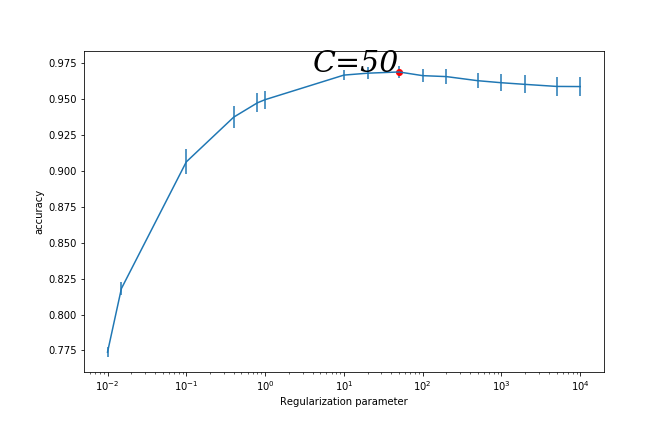
\includegraphics[width=0.45\textwidth]{figures/SVM/C.png}
		\caption{\label{fig:regularization}Erreurs de validation en fonction de paramètre de régularisation} 
	\end{center}
\end{figure}

Pourtant, le score de performance n'atteint que $ 59\% $ avec le jeu de données normalisées. Ensuite, nous entraînons le classifieur avec le jeu de données normalisé et son gradient normalisé dans le but de récupérer les informations cachées sous la série temporelle. Malheureusement, nous avons obtenu qu'une petit augmentation avec un score de performance $ 62\% $. 




%------------------------------------------------
\section{Ouverture}
L'étude de la classification des images satellites est très répandue, pour de nombreuses raisons. Elle permet de suivre l'évolution des terrains ou encore de voir les effets du réchauffement climatique. Pour comparer notre analyse à d'autres études, nous nous sommes focalisés sur l'article \cite{landClassification} \textit{Land Cover Classification of Lansat with Phenological Features Extracted from Times Series MODIS NDVI data}. Cette analyse se base aussi sur l'évolution dans le temps de la végétation, qui s'observe très bien entre saisons et la longueur des saisons. Ils évoquent aussi l'utilisation d'un logiciel \textbf{TIMESAT},  qui permet de corriger les données bruitées et s'applique très bien sur les jeux de données temporelles des images satellites, pour mettre en avant les caractéristiques de chaque classe. Les jeux de données sur les images satellites sont très souvent bruitées avec la présence de nuages ou encore de mauvaises mesures des machines. Il serait donc intéressant de poursuivre notre étude en réalisant un pré-traitement à l'aide de ce logiciel. Pour investir un peu plus le jeu de données ils font aussi référence à l'utilisation d'outils simples comme le max,min,mean et standard déviation que nous avons illustré dans la partie \ref{Analyse_explorratoire} avec les boîtes à moustache. On remarque aussi que dans l'étude, ils donnent un grande importance à la temporalité qui joue sur la classification. Les jeux de données provenant de plusieurs dates ont tendance à être plus fidèle dans la prédiction, d'autant plus si elles se prolongent sur plus d'un an, car pour une durée plus petite, les changement sont très faibles. Pour répondre à ce problème il est possible de dupliquer les données, pour donner l'illusion qu'elles sont réparties sur un plus grand espace temporel. Pour obtenir de meilleurs performances de classification il serait intéressant de réaliser les mesures dans une zone ciblée à intervalle régulier dans l'année et avec une répartition dans le temps tous les 16 jours exactement. 

%------------------------------------------------

\section{Conclusion}

Nous avons analysé un jeu de données complexe et aussi rencontré beaucoup de difficultés: bruit de donnée, manque d'information, rapport temporel inter-variables, déséquilibre de classe etc. Nous avons réussi à résoudre la plupart de ces problèmes pour finalement obtenir une précision de plus de $ 70\% $ avec des classifieurs de modèle Gaussian Naive Bayes et de modèle Random Forest. Comparé à la précision de choix aléatoire $ 16\% $ (1/6), ce résultat est vraiment acceptable.

Au cours de ce projet, nous avons acquis des connaissances plus profondes sur ce que nous avons appris dans le cours. Nous savons utiliser différentes méthodes appropriées dans un cas particulier. Appliquer ces méthodes en pratique sur des données réelles a été instructif. C'est une expérience précieuse qu'il a fallu vivre pendant un semestre de confinement, nous avons dû faire face à des difficultés de communication, mais finalement, chacun a fait la partie sur laquelle il a pu apporter une valeur ajoutée. Cela a aussi été une expérience utile au niveau collaboration internationale de communiquer et travailler à distance avec des collègues étrangers. 




%------------------------------------------------

% Annexes éventuelles 

\appendix % la commande \appendix change la numérotation des paragraphes 

\section{Code}\label{ann:code}

Le code suivant permet d'appliquer l'algorithme des K-mean et d'obtenir l'indice de rand ajusté pour évaluer son efficacité : 

\begin{minted}{python}
from sklearn.cluster import KMeans
from sklearn.metrics.cluster import adjusted_rand_score

x_quant = x.drop(columns=["class"])
km = KMeans(n_clusters=k,init="random")
km.fit(x_quant)
adjusted_rand_score(km.labels_,x['class'])
\end{minted}

Le code suivant permet d'obtenir les coefficients de Fourier pour l'analyse spectrale : 

\begin{minted}{python}
fourier_coef = []
for ligne in range(x.shape[0]):
    serie = x.iloc[ligne,2:]
    ft = np.fft.fft(serie)
    module = list(map(np.absolute,ft))
    argument = list(map(np.angle,ft))
    n = len(module)
    fourier_coef += [[module[i] for i in range(len(module)-n,len(module))]+[argument[i] for i in range(len(argument)-n,len(argument))]]
for i in range(len(fourier_coef[0])//2):
    x["fourier_coef_module"+str(i)] = list(map(lambda x:x[i],fourier_coef))
for i in range(len(fourier_coef[0])//2,len(fourier_coef[0])):
    x["fourier_coef_argument"+str(i-len(fourier_coef[0])//2)] = list(map(lambda x:x[i],fourier_coef))
\end{minted}


\bibliographystyle{plain}
\begin{thebibliography}{9}
\bibitem{landClassification} 
Kun Jia, Shunlin Liang, Xiangqin Wei, Yunjun Yao, Yingru Su5, Bo Jiang and Xiaoxia Wang
\\\textit{Land Cover Classification of Landsat Data with Phenological Features Extracted from Time Series MODIS NDVI Data}
\\Available online at \href{https://www.researchgate.net/publication/286030934_Land_Cover_Classification_of_Landsat_Data_with_Phenological_Features_Extracted_from_Time_Series_MODIS_NDVI_Data}{this URL}
\\2014-10-21

\bibitem{SVM_normalization} 
Neeraj Kumar
\\\textit{Using Support Vector Machines Effectively}
\\Available online at \href{https://neerajkumar.org/writings/svm/}{this URL}
\\August 2012
\end{thebibliography}





\end{document}
